\documentclass[10pt]{article}
\usepackage[paperwidth=198mm,paperheight=59mm,margin=1mm]{geometry}
\usepackage{newtxtext,newtxmath,tikz,pgfplots}
\pgfplotsset{compat=1.18}
\definecolor{methodblue}{HTML}{216A85}
\definecolor{controlgray}{HTML}{555555}
\definecolor{accentorange}{HTML}{A64B1D}
\pagestyle{empty}
\begin{document}\noindent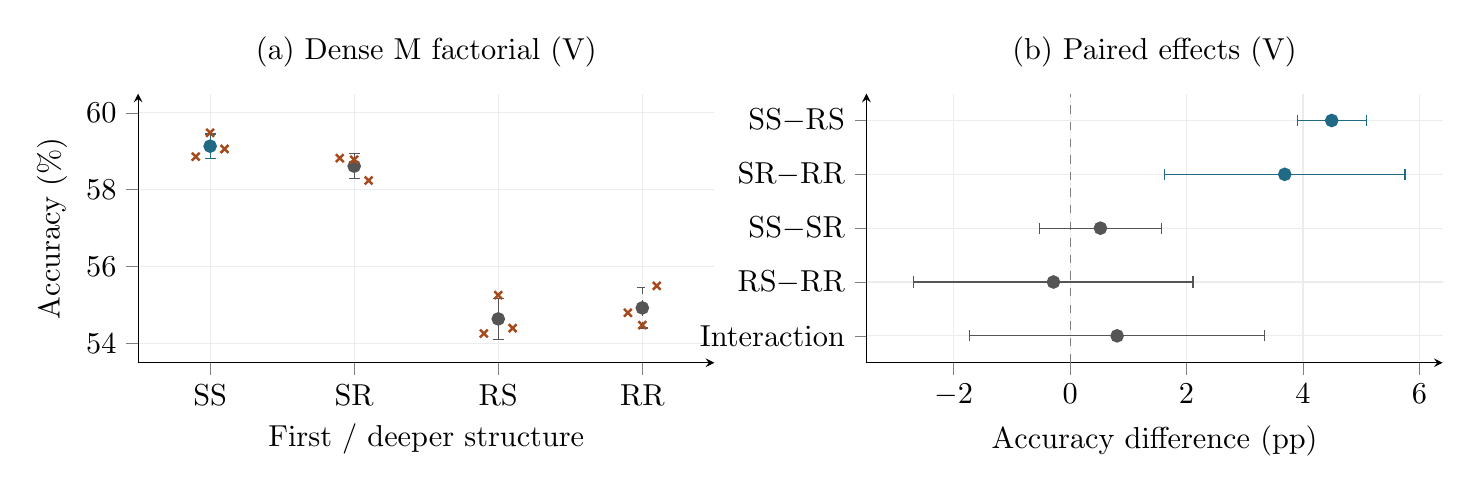
\begin{tikzpicture}
\begin{axis}[width=89mm,height=50mm,axis lines=left,tick align=outside,grid=major,grid style={gray!15},scaled ticks=false,tick label style={font=\fontsize{11}{13}\selectfont},label style={font=\fontsize{11}{13}\selectfont},title style={font=\fontsize{11}{13}\selectfont},legend style={font=\fontsize{11}{13}\selectfont,draw=none,fill=white,inner sep=1pt},title={(a) Dense M factorial (V)},xmin=-.5,xmax=3.5,ymin=53.5,ymax=60.5,xtick={0,1,2,3},xticklabels={SS,SR,RS,RR},xlabel={First / deeper structure},ylabel={Accuracy (\%)}]
\addplot+[color=methodblue,mark=*,mark size=2pt,line width=0.9pt,mark options={solid,fill=methodblue,draw=methodblue},only marks,error bars/.cd,y dir=both,y explicit] coordinates {(0,59.133332) +- (0,0.31643868)};
\addplot+[color=accentorange,mark=x,mark size=2pt,line width=0.9pt,mark options={solid,fill=accentorange,draw=accentorange},only marks] coordinates {(-0.1,58.859999)(0,59.479999)(0.1,59.059999)};
\addplot+[color=controlgray,mark=*,mark size=2pt,line width=0.9pt,mark options={solid,fill=controlgray,draw=controlgray},only marks,error bars/.cd,y dir=both,y explicit] coordinates {(1,58.613332) +- (0,0.32393412)};
\addplot+[color=accentorange,mark=x,mark size=2pt,line width=0.9pt,mark options={solid,fill=accentorange,draw=accentorange},only marks] coordinates {(0.9,58.819998)(1,58.779999)(1.1,58.239998)};
\addplot+[color=controlgray,mark=*,mark size=2pt,line width=0.9pt,mark options={solid,fill=controlgray,draw=controlgray},only marks,error bars/.cd,y dir=both,y explicit] coordinates {(2,54.639999) +- (0,0.54147922)};
\addplot+[color=accentorange,mark=x,mark size=2pt,line width=0.9pt,mark options={solid,fill=accentorange,draw=accentorange},only marks] coordinates {(1.9,54.259999)(2,55.259998)(2.1,54.399999)};
\addplot+[color=controlgray,mark=*,mark size=2pt,line width=0.9pt,mark options={solid,fill=controlgray,draw=controlgray},only marks,error bars/.cd,y dir=both,y explicit] coordinates {(3,54.926666) +- (0,0.5216639)};
\addplot+[color=accentorange,mark=x,mark size=2pt,line width=0.9pt,mark options={solid,fill=accentorange,draw=accentorange},only marks] coordinates {(2.9,54.799999)(3,54.479999)(3.1,55.499999)};
\end{axis}
\begin{axis}[width=89mm,height=50mm,axis lines=left,tick align=outside,grid=major,grid style={gray!15},scaled ticks=false,tick label style={font=\fontsize{11}{13}\selectfont},label style={font=\fontsize{11}{13}\selectfont},title style={font=\fontsize{11}{13}\selectfont},legend style={font=\fontsize{11}{13}\selectfont,draw=none,fill=white,inner sep=1pt},at={(9.25cm,0)},anchor=south west,title={(b) Paired effects (V)},xmin=-3.5,xmax=6.4,ymin=-.5,ymax=4.5,ytick={0,1,2,3,4},yticklabels={{Interaction},{RS$-$RR},{SS$-$SR},{SR$-$RR},{SS$-$RS}},xlabel={Accuracy difference (pp)}]
\draw[dashed,gray] (axis cs:0,-.5)--(axis cs:0,4.5);
\addplot+[color=methodblue,mark=*,mark size=2pt,line width=0.9pt,mark options={solid,fill=methodblue,draw=methodblue},only marks,error bars/.cd,x dir=both,x explicit] coordinates {(4.4933336,4) +- (0.59273204,0)};
\addplot+[color=methodblue,mark=*,mark size=2pt,line width=0.9pt,mark options={solid,fill=methodblue,draw=methodblue},only marks,error bars/.cd,x dir=both,x explicit] coordinates {(3.6866661,3) +- (2.0660698,0)};
\addplot+[color=controlgray,mark=*,mark size=2pt,line width=0.9pt,mark options={solid,fill=controlgray,draw=controlgray},only marks,error bars/.cd,x dir=both,x explicit] coordinates {(0.52000042,2) +- (1.0433379,0)};
\addplot+[color=controlgray,mark=*,mark size=2pt,line width=0.9pt,mark options={solid,fill=controlgray,draw=controlgray},only marks,error bars/.cd,x dir=both,x explicit] coordinates {(-0.28666703,1) +- (2.3978461,0)};
\addplot+[color=controlgray,mark=*,mark size=2pt,line width=0.9pt,mark options={solid,fill=controlgray,draw=controlgray},only marks,error bars/.cd,x dir=both,x explicit] coordinates {(0.80666745,0) +- (2.531546,0)};
\end{axis}
\end{tikzpicture}\end{document}
